\documentclass[10pt]{beamer}

\usepackage[T2A]{fontenc}
\usepackage[utf8]{inputenc}
\usepackage[russian,english]{babel}
\usepackage{subfig}
\usepackage[noend]{algorithm,algpseudocode}
\usepackage{amsmath}

\usepackage{booktabs}
\usepackage[scale=2]{ccicons}

\usepackage{pgfplots}
\usepgfplotslibrary{dateplot}

\usepackage{xspace}
\newcommand{\TODO}[1]{\textbf{\textcolor{red}{TODO: #1}}}


\algblockdefx{MRepeat}{EndRepeat}{\textbf{repeat}}{}
\algnotext{EndRepeat}

\algrenewcommand\alglinenumber[1]{\footnotesize #1}
\DeclareMathOperator{\rank}{rank}
\DeclareMathOperator{\sign}{sign}

\newcounter{mycounter}

\newcommand{\myparagraph}{\stepcounter{mycounter}\paragraph{\arabic{mycounter}}}

\title{Лекция 13}
\subtitle{Композиции алгоритмов}

\begin{document}

\section{Разбор летучки}

\maketitle

\section{Мотивация}

\section{Где уже видели композиции?}

\begin{frame}{Постановка задачи}
  ${X^l = (x_i, y_i)_{i = 1}^l}$ -- обучающая выборка\\
  $b:X \rightarrow R$ --- базовый алгоритм\\
  $C:R \rightarrow Y$ --- решающее правило\\
  $R$ --- пространство оценок.
  \bigbreak
  Искомый алгоритм: $a(x) = C(b(x))$\\
\end{frame}

\begin{frame}{Примеры}
  \begin{enumerate}
    \item Классификация (2 класса): \qquad $a(x) = \sign(b(x))$\\      
      $b: X \rightarrow \mathbb{R} \qquad C(b) = \sign(b)$
    \item Классификация (M классов): \qquad $a(x) = \arg\max\limits_{y \in Y} (b_y(x))$\\      
      $b: X \rightarrow \mathbb{R}^M \qquad C(b_1, \dots, b_M) = \arg\max\limits_{y \in Y}(b_y)$
    \item Регрессия\\
      $C(b) = b$      
  \end{enumerate}
\end{frame}

\begin{frame}{Определение композиции}
  Композиция базовых алгоритмов $b_1, \dots, b_T$\\
  \bigbreak
  $a(x) = C(F(b_1(x), \dots, b_T(x)))$\\
  $F: R^T \rightarrow R$ -- корректирующая операция
\end{frame}

\begin{frame}{Примеры}
  \begin{enumerate}
    \item Простое голосование\\
      $$F(b_1(x), \dots, b_T(x)) = \frac{1}{T}\sum\limits_{t=1}^{T} b_t(x)$$
    \item Взвешенное голосование\\
      $$F(b_1(x), \dots, b_T(x)) = \sum\limits_{t=1}^{T} \alpha_t b_t(x)$$
    \item Смесь алгоритмов\\
      $$F(b_1(x), \dots, b_T(x)) = \sum\limits_{t=1}^{T} g_t(x) b_t(x)$$      
  \end{enumerate}
\end{frame}

\section{Простое голосование}

\begin{frame}{Теорема Кондорсе "о жюри присяжных"}
  Если каждый член жюри присяжных имеет независимое мнение, и если вероятность правильного решения члена жюри больше 0.5, то тогда вероятность правильного решения присяжных в целом возрастает с увеличением количества членов жюри и стремится к единице.   
\end{frame}


\begin{frame}{Простое голосование}
  $$F(b_1(x), \dots, b_T(x)) = \frac{1}{T}\sum\limits_{t=1}^{T} b_t(x)$$
  \bigbreak
  \pause
  $$a(x) = \sign \left( \sum\limits_{t=1}^{T} b_t(x) \right)$$
  \bigbreak
  \pause
  Если каждый из $b_t$ лучше случайного гадания и $b_1, \dots, b_T$ достаточно различны, то композиция может работать лучше.
\end{frame}

\begin{frame}{Достаточно различны?}
  \begin{itemize}
    \item Настройка по случайным подвыборкам
    \item Обучение по случайным подмножествам признаков
    \item Использование различных начальных приближений 
    \item Использование различных моделей
  \end{itemize}
\end{frame}

{\foot{Bagging, Bootstrap aggregating}
\begin{frame}{Бэггинг}
    \alert{Идея}: обучим $b_t$ независимо по случайным подвыборкам длины $l$ с повторениями.\\
    Доля объектов, которые попадут в выборку $\approx 0.63$
\end{frame}
}

\begin{frame}{Бэггинг}
    Бэггинг позволяет снизить дисперсию (variance) обучаемого классификатора. 
    \bigbreak
    \pause
    Бэггинг эффективен на малых выборках, когда исключение даже малой части обучающих объектов приводит к построению существенно различных базовых классификаторов.
%    \\
%    \bigbreak
%    Ошибка каждого классификатора:\\
%    $$\varepsilon_i(x) = b_i(x) - y(x)$$
%    Матожидание:\\
%    $$E_x (b_i(x) - y(x))^2 = E_x \varepsilon_i(x)^2$$
\end{frame}

{\foot{RSM, Random Subspace Method}
\begin{frame}{Метод случайных подпространств}
    \alert{Идея}: обучим $b_t$ независимо по случайным подмножествам $n'$ признаков.\\
\end{frame}
}

\begin{frame}{Алгоритм}
  	\begin{algorithmic}[1]
    \Function{bagging\_rsm}{$X^l$, $T$, $l'$, $n'$, $\varepsilon_1$, $\varepsilon_2$}
      \For {$t = 1, \dots, T$}
        \State $U_t$ -- случайное подмножество $X^l$ длины $l'$
        \State $F_t$ -- случайное подмножество признаков длины $n'$
        \State $b_t = \mu (F_t, U_t)$
        \If {$Q(b_t, U_t) > \varepsilon_1$ или $Q(b_t, X^l \setminus U_t) > \varepsilon_2$}
          \State не включать $b_t$ в композицию
        \EndIf
      \EndFor
    \EndFunction
  \end{algorithmic}
\end{frame}

{\foot{Random forest}
\begin{frame}{Случайный лес}
  Бэггинг над решающими деревьями.\\
  \bigbreak
	Голосование деревьев классификации, $Y = \left\{ -1, +1 \right\}$\\
	$a(t) = Majority(b_t(x))$%\sign \frac{1}{T} \sum\limits_{t=1}^T b_t(x)$\\
	\begin{enumerate}[--]
  	  \item Каждое дерево $b_t(x)$ обучается по случайной выборке с повторениями
	  \item В каждой вершине предикат выбирается из случайного подмножества $n$ предикатов
	\end{enumerate}
\end{frame}
}

\section{Взвешенное голосование}

{\foot{Boosting}
\begin{frame}{Бустинг}
  $Y = \{\pm 1\}$, \qquad $b_t: X\rightarrow \{-1, 0, +1\}$, \qquad $C(b) = \sign(b)$\\
  $b_t(x) = 0$ -- отказ от классификации\\
  \bigbreak
  \pause
  $a(x) = \sign\left(\sum\limits_{t=1}^{T} \alpha_t b_t(x)\right)$\\
  \bigbreak
\end{frame}
}

{\foot{Boosting}
\begin{frame}{Бустинг}
  \alert{Идея}: Фиксируем $\alpha_1 b_1(x) \dots \alpha_{t-1} b_{t-1}(x)$ при добавлении $b_t$
  \bigbreak
  \pause
  $b_1 = \arg\min\limits_{b} Q(b, X^l)$\\
  $b_2 = \arg\min\limits_{b, F} Q(F(b_1, b), X^l)$\\
  $\dots$\\
  $b_t = \arg\min\limits_{b, F} Q(F(b_1, \dots, b_{t-1}, b), X^l)$
\end{frame}
}

\begin{frame}{Функционал качества}  
  Функционал качества композиции:\\
  $Q_T = \sum\limits_{i=1}^l \mathcal{L}(\sum\limits_{t=1}^{T} \alpha_t b_t(x_i), y_i)  = 
  \sum\limits_{i=1}^l \left[ y_i \sum\limits_{t=1}^{T} \alpha_t b_t(x_i) < 0 \right] \rightarrow \min\limits_{\alpha, b}$
  \bigbreak
  \pause
  Оценка функционала сверху:\\
  $Q_T \leq \hat{Q}_T = \sum\limits_{i=1}^l \underbrace{ \exp \left( -y_i \sum\limits_{t=1}^{T-1} \alpha_t b_t(x_i) \right) }_{w_i} \exp(-y_i \alpha_T b_T(x_i))\rightarrow \min\limits_{\alpha, b}$\\
\end{frame}

\begin{frame}{Бустинг}  
  Нормируем веса:\\
  $u_i = w_i / \sum\limits_{j=1}^l w_j$
  \bigbreak
  Взвешенное число ошибочных классификаций:\\
  $N(b, U^l) = \sum\limits_{i=1}^l u_i [b(x_i) = -y_i]$
  \bigbreak
  Взвешенное число правильных классификаций:\\
  $P(b, U^l) = \sum\limits_{i=1}^l u_i [b(x_i) = y_i]$
\end{frame}

\begin{frame}{Adaboost}
  $B$ -- семейство базовых алгоритмов.\\
  \bigbreak
  Пусть для любого нормированного вектора весов $U^l$ существует алгоритм $b \in B$, классифицирующий выборку немного лучше, чем наугад $P(b, U^l) > N (b, U^l)$. \\
  Минимум функционала $Q_T$ достигается при:\\
  $$b_T = \arg\max\limits_{b \in B} \sqrt{P(b, U^l)} - \sqrt{N(b, U^l)}$$
  $$\alpha_T = \frac{1}{2} \ln \frac{P(b_T, U^l)}{N(b_T, U^l)}$$
\end{frame}

\begin{frame}{Алгоритм}
  \begin{algorithmic}[1]
    \Function{adaboost}{$X^l$, $T$}
      \State Инициализировать $w_i = 1 / l, \qquad i=1, \dots, l$
      \For {$t = 1, \dots, T$}
        \State $b_t = \arg\max\limits_{b \in B} \sqrt{P(b, U^l)} - \sqrt{N(b, U^l)}$
        \State $\alpha_t = \frac{1}{2} \ln \frac{P(b_T, U^l)}{N(b_T, U^l)}$
        \State $w_i = w_i \exp (- \alpha_t y_i b_t(x_i)) \qquad i=1, \dots, l$
        \State $u_i = w_i / \sum\limits_{j=1}^l w_j$
      \EndFor
    \EndFunction
  \end{algorithmic}
\end{frame}

\begin{frame}{Рекоммендации}
  \begin{itemize}
    \item Чаще всего в качестве базовых классификаторов используются решающие деревья
    \item Для SVM бустинг не эффективен     
  \end{itemize}
\end{frame}

\begin{frame}{Наблюдения}
  \begin{itemize}[<+->]
    \item[+] Хорошая обобщающая способность
    \item[+] Простота реализации
    \item[+] Накладные расходы на построение не велики
    \bigbreak
    \item[--] Склонен к переобучению при наличии большого количества шума в данных
    \item[--] Требует большой обучающей выборки
    \item[--] Жадность приводит к неоптимальности
  \end{itemize}
\end{frame}

\begin{frame}{Stacking}
    \centering
    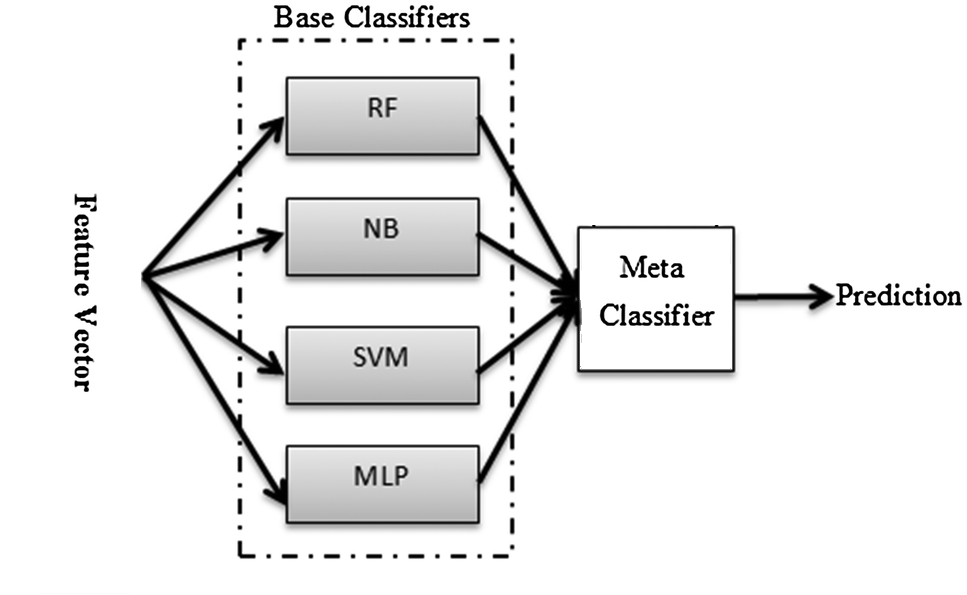
\includegraphics[width=0.9 \textwidth, keepaspectratio]{images/stacking}
\end{frame}

\begin{frame}{Почему эти подходы работают}
  \begin{enumerate}
    \item Бэггинг уменьшает разброс
    \item Бустинг уменьшает разброс и смещение
    \item Чем сильнее коррелируют базовые алгоритмы, тем менее эффективны композиции
  \end{enumerate}
\end{frame}

\begin{frame}[standout]
  Вопросы?
\end{frame}

\appendix

\end{document}

\end{document}